\documentclass{article} % For LaTeX2e
\usepackage{11785_project,times}
\usepackage{hyperref}
\usepackage{url}
\usepackage{graphicx}

\usepackage{subcaption}

\title{Visual Attention: Scanpath Generation Using Deep learning}


\author{
Daniel Marew \\
\texttt{dmarew@andrew.cmu.edu} \\
}

\begin{document}
\maketitle

\begin{abstract}
A number of visual attention models aimed at predicting human eye fixations  have been proposed. The majority of these, focus solely on predicting saliency maps that represent the likelihood a location in an image being fixated on. They are not concerned with generating temporally ordered human-like sequences of saccades. To address this gap, we present a generative model based on a deep recurrent architecture that
predicts human visual scan-path gaze sequences for a given image in  free viewing task. The model is trained with real-world human eye-tracking data to maximize the likelihood of generating a human like scanpath given an image. This research was conducted with in a seven week period for six units of credit.
\end{abstract}

\section{Introduction}

Research in the field of visual cognition has shown that when humans observe a scene, they tend to focus on different regions of the image with different levels of intensity. They gaze more on salient and relevant parts guided by visual attention mechanisms (\cite{rensink_2000}). Understanding and modeling these human visual attentional mechanisms is an active area of research in the fields of neuroscience and computer vision due to their relevance in variety of practical tasks such as  as object recognition (\cite{paletta_fritz_2007}), face recognition (\cite{goodrich_arel_2012}),  visual search in surveillance (\cite{minut_mahadevan_2001}), autonomous navigation (\cite{borji_ahmadabadi_araabi_2009}), among others.

There are two main ways of representing visual attention saliency information: saliency maps and scanpaths. Saliency maps represent the likelihood a location in an image being fixated on. It is often represented as a single channel image obtained by aggregating salient points and then convolving each point with a Gaussian kernel. Scanpaths, on the other hand, are defined by the location of the fixation points and the dwell time the eye fixates on a point between saccades. They are temporally ordered sequences of saccades. 

Most computational models of visual attention focus solely on predicting saliency maps and are not concerned with generating temporally ordered human-like sequences of saccades, i.e scanpaths. To address this gap, we present a generative model based on a deep recurrent architecture that
predicts human visual scan-path gaze sequences for a given image in  free viewing task.

The remaining of the work is organized as follows. Section 2 reviews computational visual attention models for both saliency map and scanpath modeling. Section 3 presents our scanpath model, a deep neural network based on encoder-decoder architecture (convolutional neural network (CNN) encoder and long short term memory (LSTM) decoder). Section 4 describes scanpath binning (a technique we use to reduce the complexity of our problem), the dataset used, the training details of the network and the evaluation metric. Section 5 includes the experiments and results of the presented technique. Finally, Section 6 closes the report by stating the main conclusions and future works that could be done to improve the current performance of our model.

This research was conducted with in a seven week period for six units of credit.

\begin{figure}
\begin{subfigure}{.33\textwidth}
  \centering
  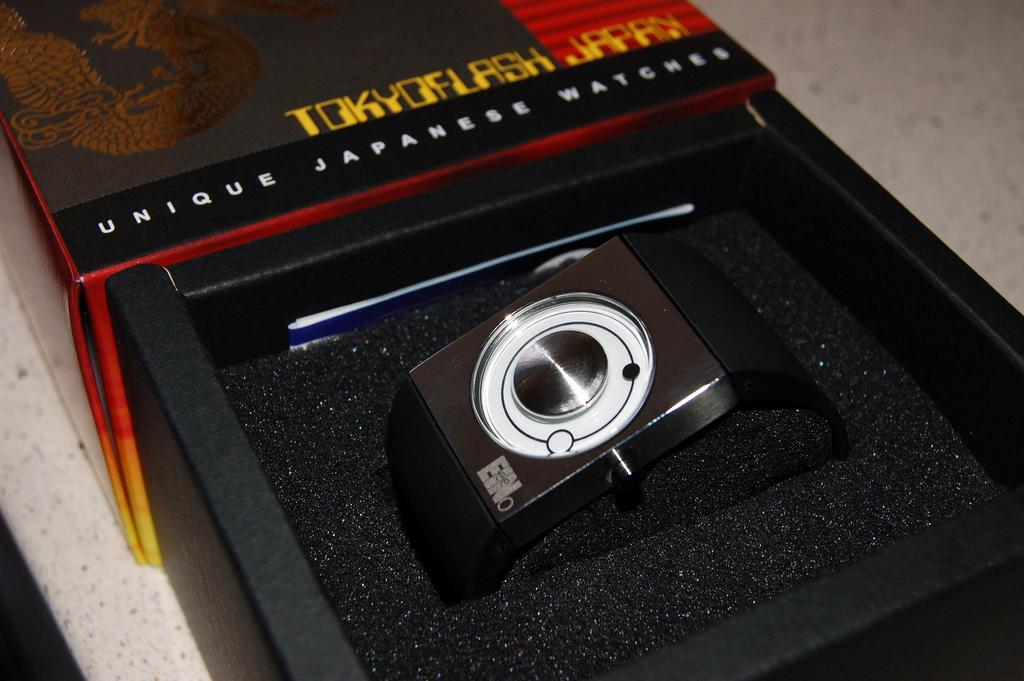
\includegraphics[width=.8\linewidth]{input.jpeg}
  \caption{Image}
  \label{fig:sfig1}
\end{subfigure}%
\begin{subfigure}{.33\textwidth}
  \centering
  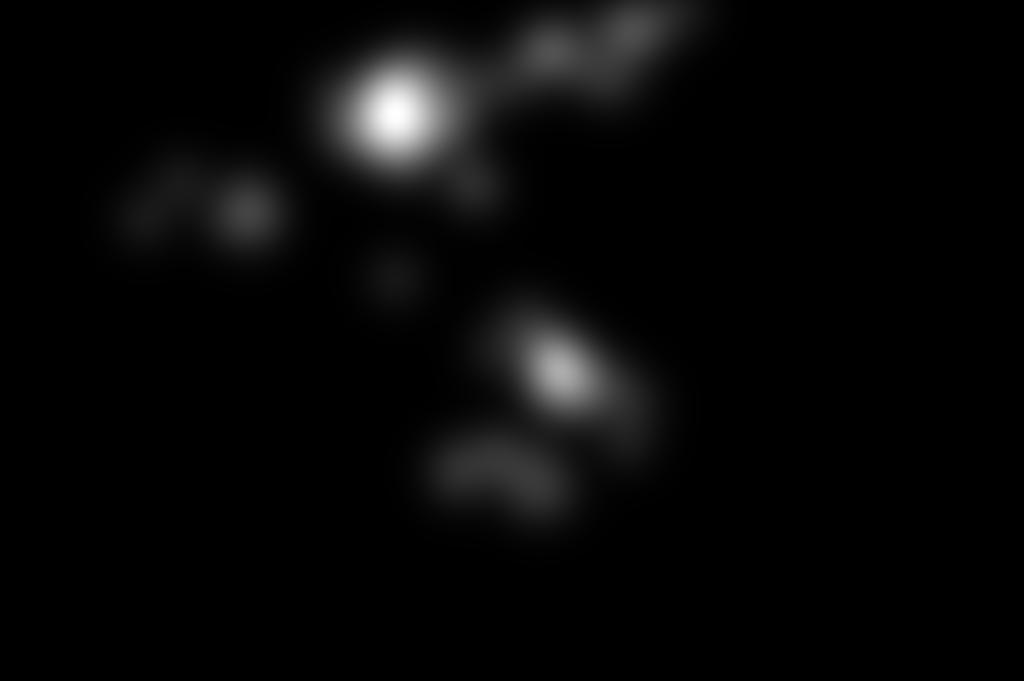
\includegraphics[width=.8\linewidth]{map.jpg}
  \caption{Saliency Map}
  \label{fig:sfig2}
\end{subfigure}
\begin{subfigure}{.33\textwidth}
  \centering
  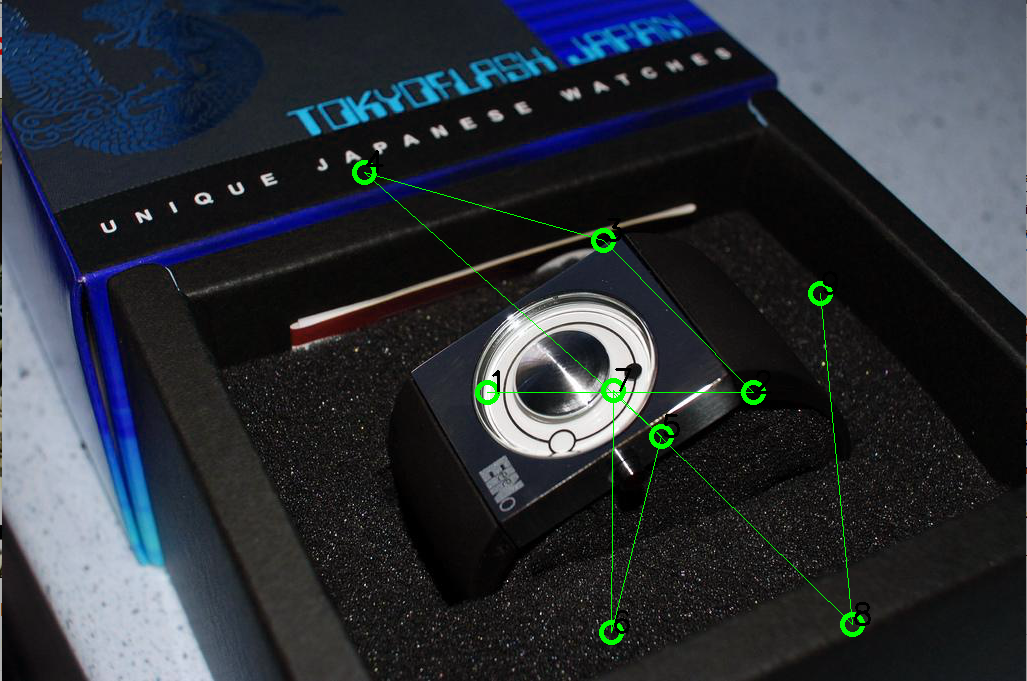
\includegraphics[width=.8\linewidth]{scanpath.png}
  \caption{Scanpath}
  \label{fig:sfig3}
\end{subfigure}
\caption{Sample images taken from \cite{Judd_2009} dataset (a) shows the input image. (b) is the ground truth saliency map for (a). (c) shows scanpath of one of the subjects. }
\label{fig:fig}
\end{figure}

\section{Computational Models Of Visual Attention}
\subsection{Saliency Map Modeling}
In their  seminal works on visual attention \cite{koch_ullman_1987},
\cite{tsotsos_culhane_wai_lai_davis_nuflo_1995} and \cite{itti_koch_niebur_1998} introduced predictive biologically inspired models based on a bottom-up computational model that extracted low-level visual features such as intensity, color, orientation, texture and motion at multiple scales. Since then,  a number of saliency map prediction algorithms have been proposed, some using information theoretic principles (\cite{bruce_tsotsos_2007}), others with data driven approaches using machine learning algorithms. For example, \cite{Judd_2009} introduced an approach that used low, mid and high-level image features to define salient
locations. These features were used in combination with a linear support vector machine to train a saliency model. Recently, since their resurgence, many of the algorithms proposed by the community have been based on deep learning networks mainly convolutional neural networks (CNNs) which  have been shown to capture high-level features especially in the domain of image classification. For instance, \cite{Kummerer_2017_ICCV} introduced a model that predicts saliency maps based on deep neural network features trained on object recognition which set a new state-of-the art in saliency map prediction on the MIT300 hold-out benchmark. 

\cite{DBLP:journals/corr/CorniaBSC16a} went beyond the standard approaches to saliency prediction, in which gaze maps are computed with a feed-forward network, and presented a novel model which can predict accurate saliency maps by incorporating neural attentive mechanisms. The core of their solution relied on  a Convolutional LSTM (Long Short Term Memory) that focuses on the most salient regions of the input image to iteratively refine the predicted saliency map. Additionally, they also showed that the center bias present in human eye fixations can be tackled by learning  a set of prior maps generated with Gaussian functions.

\subsection{Scanpath Modeling}
Most attention models, including the aforementioned once, are only concerned with the related task of saliency map modeling. That said, there have been some attempts to model scanpath generation where by scanpaths are defined by the location of the fixation points and the dwell time the eye fixates on a point between saccades.

For example, \cite{jiang_boix_roig_xu_gool_zhao_2016} presented a method for modeling the human visual scanpath that is learned from recorded human eye tracking data. They used Least-Squares Policy Iteration to learn a visual exploration policy that mimics the recorded eye-fixation examples. The model uses a different set of parameters for the different stages of visual exploration to capture the importance of the cues during the scan-path

\cite{DBLP:journals/corr/AssensMGO17} proposed a deep convolutional neural network (DCNN) that predicts
a saliency volume,  a representation of spatial and temporal saliency information for images, for a given input image. They also presented a heuristic mechanism for  generating scanpaths over  360-degree images by sampling the predicted saliency volumes.

\cite{DBLP:journals/corr/abs-1711-10959} showed that their model, STAR-FC, a novel multi-saccade generator based on a central/peripheral integration of deep learning-based saliency and lower-level feature based saliency, can successfully predict human patterns of fixation with equivalent accuracy and quality compared to what can be achieved by using one human sequence to predict another, i.e the similarity between a scanpath generated by the model and a human scanpath, is comparable to the similarity between two scanpaths generated by two independent humans. 

\section{Scanpath Model}
\begin{figure}[h]
    \centering
    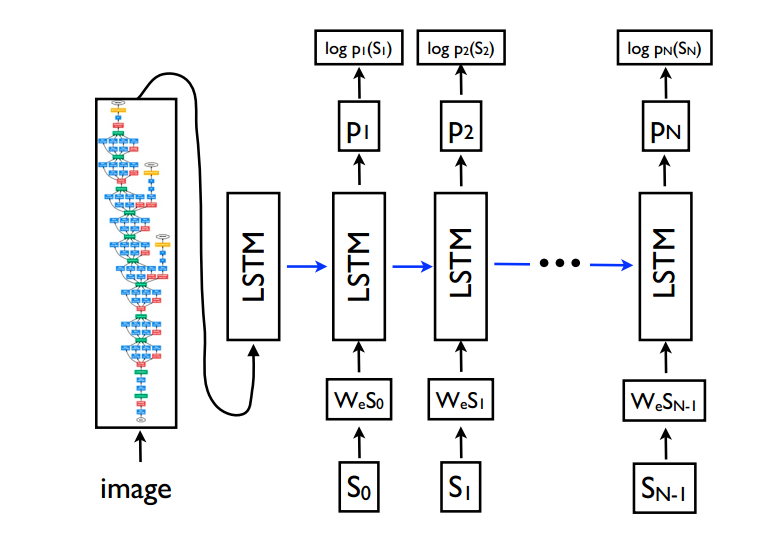
\includegraphics[scale=0.5]{captioning.png}
    \caption{System Architecture \cite{DBLP:journals/corr/VinyalsTBE14}. The image goes through a CNN, ResNet152 in particular, the encoder. The resulting high dimensional vector feature representation is then given to an LSTM, the decoder. The LSTM model is trained to predict each fixation point of the scanpath after it has seen this high dimensional feature vector represention of the image as well as all preceding fixation points. The figure shows the unrolled form of the LSTM  such that all LSTMs share the same parameters and the output $m_t-1$ of the LSTM at time $t-1$ is fed to the LSTM at time $t$.   }
    \label{fig:arch}
\end{figure}
The problem of image captioning is similar to the scanpath generation problem in the sense that both are trying predict a sequence of items: words and fixation points(and dwell time) respectively, given an image. We hypothesize that an architecture that works for one works for the other. The goal of this report is to validate this and show that such an architecture can generate scanpaths that are comparable to those of  human observers. In particular, we developed an architecture that is inspired by an image captioning generative deep learning architecture described in \cite{DBLP:journals/corr/VinyalsTBE14}. % which outputs a caption, a sequence of words, from a vocabulary of English words, given an image.
They showed that the probability of correct captioning can be directly maximized given the image by using the following formulation.
\begin{equation}
    \theta^{*} = \arg\max_{\theta}\sum_{(I, S)} \log p(S|I,\theta) 
\end{equation}
where $\theta$ are the parameters of the model, $I$ is an image, and $S$ its correct transcription.
They used chain rule to model the joint probability over $\{S_0, \dots \dots, S_N\}$ where $N$ is the length of the caption. 
\begin{equation}
    \log p(S|I) = \sum_{t=0}^{N}\log p(S_t|I, S_{0}, \dots S_{t-1})
\end{equation}

They then used a Recurrent Neural Network (RNN), a LSTM in particular, to model $p(S_t| I, S0,\dots \dots, S_{t-1})$ where the variable number
of words are conditioned upon up to $t- 1$ is expressed by a fixed length hidden state or memory $h_t$.

In our case, instead of outputting a sequence of words, the model outputs a scanpath, a sequence of fixation points and their dwell times. The model architecture is depicted in Fig. \ref{fig:arch}. It has two main parts. An encoder: a convolutional neural network (CNN) and a decoder in the form of a long short term memory network (LSTM) .

We use the CNN to extract high level image features. It is a 152 layer network called Resnet152 (\cite{DBLP:journals/corr/HeZRS15}) which is trained for image classification task and has been shown to generalize to other tasks by means of transfer learning. %The input image has to be resized to 224x224 to work Resnet152.

To generate scanpaths, we use an LSTM model trained to predict each
fixation of the scanpath after it has seen the image as well
as all preceding fixations as defined by $p(S_t| I, S0,\dots \dots, S_{t-1})$. The overall scanpath generation is as follows:

$$x_{-1} = CNN(I)$$
$$x_{t} = W_eS_t, t\in\{0, \dots \dots, N-1\}$$
$$p_{t+1} = LSTM(x_t), t\in\{0, \dots \dots, N-1\}$$
where $p_{t+1}$ is a probability distribution over all scanpath bins (our vocabulary), $W_e$ are the weights of our fixation embedding and $x_{-1}$ is a vector form feature representation extracted from the input image by the CNN.

To learn the parameters of the LSTM and fixation embedding $W_e$ we use   the sum of the negative log likelihood, defined below, as a divergence function.
\begin{equation}
 L(I|S) = -\sum_{t=1}^{N} \log p_{t}(S_t)    
\end{equation}

\section{Emperical Investigation}
\subsection{Scanpath Binning}
A scanpath is defined by the location of the fixation points and the dwell time the eye fixates on a point between saccades. To simplify the training of our network, we transform this representation such that each fixation point $(x, y, t)$ is represented by a single number. This can be achieved by spatially and temporally binning the fixations and assigning a unique number to each bin. The binning resolution we use is 64x64x8 that is, 64 bins for width and height and 8 for dwell time. So for example, an input image with size 1024x1024 will have 32768(64x64x8) 16x16x8  bins which is close to the vocabulary size in many LSTM based language models. That means we can predict the location of a fixation with a maximum error margin of $\pm 8$ pixels in both x and y dimensions with in a bin.
\begin{equation}
S=\big\{(x_1, y_1, t_1), (x_2, y_2, t_2), \dots , (x_n, y_n)\big\} \Rightarrow \big\{S_1, S_2,\dots, S_n\big\}
\end{equation}
Besides simplifying the training process, scanpath binning also greatly reduces the complexity of our problem. For instance, in the previous example, had we used pixel level binning resolution we would have 8,388,608 (1024x1024x8) 1x1x8 bins which is too complex to be modeled by our simple architecture.

Once we have the bins, each scanpath is transformed into a sequence of numbers by replacing each fixation$(x, y, t)$ with the unique number corresponding to the grid cell the fixation falls in.

During inference, i.e when generating a scanpath, the sequence of numbers that represent the scanpath are transformed back to their original representation. This is done by first computing summary statistics, mean ($\mu$) and standard deviation ($\sigma$), for each bin over the training data. That is, each bin has a mean $x$ location, $y$ location and mean dwell time and corresponding standard deviations. We then fit Gaussian distributions $N(\mu, \sigma)$ for each dimension $(x, y, t)$ and sample from them.

\begin{figure}[!htb]
\minipage{0.32\textwidth}
  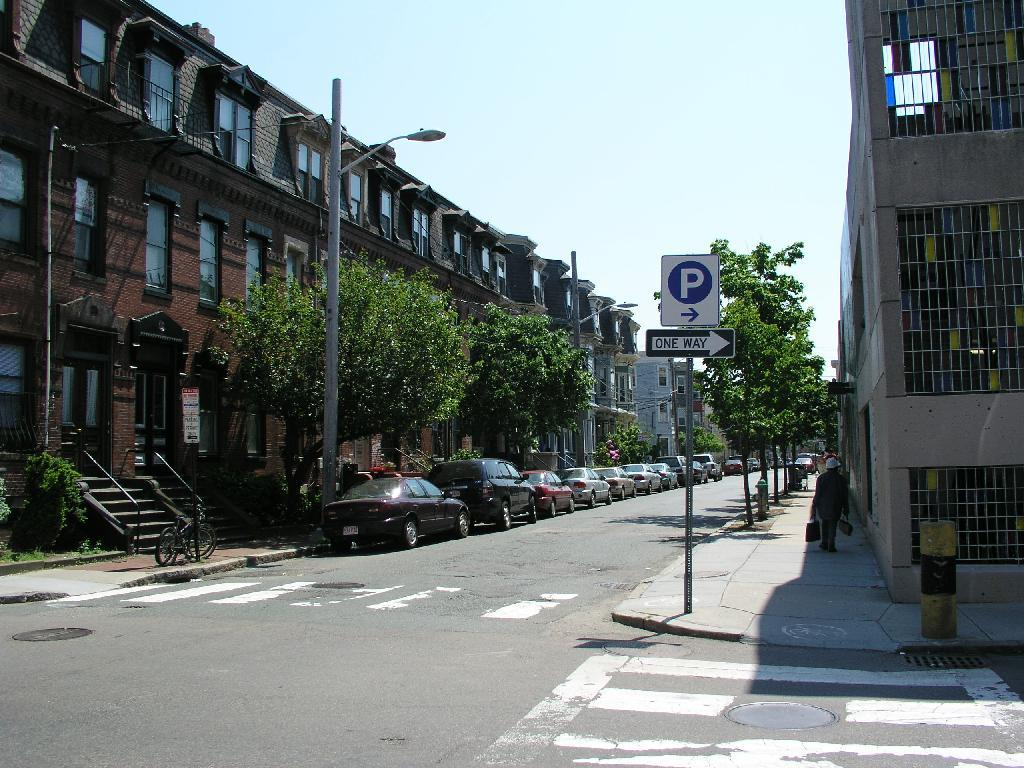
\includegraphics[width=\linewidth]{dataset.jpeg}
  \caption{Sample stimulus from \cite{Judd_2009}}\label{fig:dataset}
\endminipage\hfill
\minipage{0.32\textwidth}
\begin{tabular}{ |c|c|c|c|c|c|} 
 \hline
  $x$ & $y$ & dwell time(sec)\\ 
  \hline
499 &378& 0.334\\ 
502 &449& 0.096\\
675 &327& 0.579\\ 
686 &287& 0.725\\ 
505 &354& 0.546\\ 
477 &477& 0.517\\ 
 \hline

\end{tabular}
\caption{Eye tracking data from first subject for stimulus in figure \ref{fig:dataset}}
\endminipage\hfill
\minipage{0.32\textwidth}
\begin{tabular}{ |c|c|c|c|c|c|} 

 \hline
  $x$ & $y$ & dwell time(sec)\\ 
 \hline
 516 & 373&0.263 \\
 636 &317&0.129 \\
 655 &314& 0.229\\
 433 &464&0.250\\ 
 249 &428&0.080\\ 
 742&424&0.308\\
 797&468&0.087\\
 903&276&0.155\\
 895&71&0.420\\
 894&316&0.32\\
 \hline
\end{tabular}
\caption{Eye tracking data from second subject for stimulus in figure \ref{fig:dataset}}
\endminipage
\end{figure}

\subsection{Dataset}
We trained and evaluated our model over the MIT1003 dataset (\cite{Judd_2009}) which contains 1003 images and their corresponding eye tracking data from 15 subjects for  a free viewing task. This dataset was chosen due to several positive attributes mainly the fact that it has various types of object categories and by far is the largest free-viewing eye-tracking dataset available for natural images.
%Thesalient points over the image are usually aggregated and represented in a saliency map, a single channel image obtainedby convolving each point with a Gaussian kernel.

\subsection{Training Details}
One of the main challenges when training deep learning networks on small datasets such as MIT1003 is over-fitting. To mitigate this problem, we  employ different regularization techniques. During training, we freeze the weights of the pretrained convolutional neural network (the encoder) so that we only  train the LSTM part of the network. We also have a batch normalization layer (\cite{DBLP:journals/corr/IoffeS15} ) after the last layer of The CNN that acts as a regularizer. The weights of the embedding and linear layers of the decoder are initialized with random numbers sampled from a uniform distribution between -0.1 and 0.1 and the bias of the linear layer is initialized with zero. The model is trained for 50 epochs using ADAM optimizer (\cite{DBLP:journals/corr/KingmaB14} ) with learning rate $=1e^{-3}$, $\beta_1=0.9$,  $\beta_2=0.999$, $eps=1e^{-8}$ with no weight decay.

%\begin{figure}[!htb]
%\minipage{0.32\textwidth%}
%  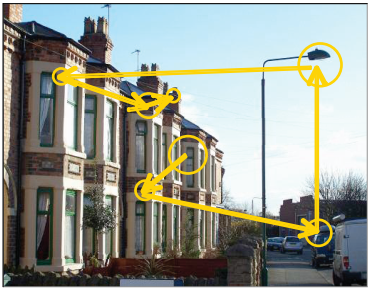
\includegraphics[width=\linewidth]{scan1.png}
 % \caption{Scanpath 1 \cite{Anderson2015} }\label{fig:scan1}
%\endminipage\hfill
%\minipage{0.32\textwidth}
 % 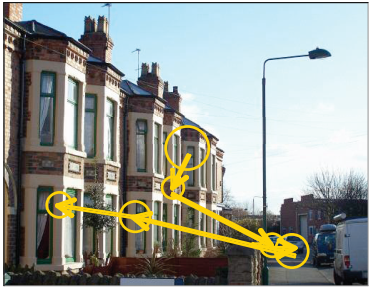
\includegraphics[width=\linewidth]{scan2.png}
  %\caption{Scanpath 2 \cite{Anderson2015}}\label{fig:scan2}
%\endminipage\hfill
%\minipage{0.32\textwidth}%
  %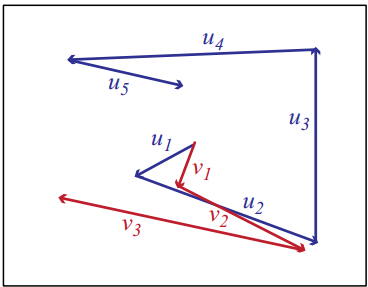
\includegraphics[width=%\linewidth]{simple.png}
  %\caption{Multimatch simplified scanpaths %\cite{Anderson2015}}\label{fig:scan3}
%\endminipage
%\end{figure}
\subsection{Evaluation Metric}
The evaluation metrics we use to measure the performance our model are computed by a method called MultiMatch (\cite{7ccdec072dc945c4a0138a73aedd0132} ).
It is a pairwise similarity measure that allows a detailed comparison of scanpaths by capturing their different spatial and temporal characteristics, namely their shape, direction, length, position and duration. MultiMatch starts out by simplifying the scanpaths 
which involves combining iteratively successive fixations if they are within a given distance or
within a given directional threshold of each other (\cite{Anderson2015} ). This simplification process helps in reducing the complexity of the scanpaths while preserving their spatial and temporal structure. After this simplification, scanpaths are temporally aligned to each other based
on their shape using a dynamic programming algorithm. Then five similarity metrics are computed from the simplified and temporally aligned scanpaths.

The five similarity metrics are the following. 
\begin{enumerate}
\item Vector  similarity is computed as the vector difference between aligned saccade pairs and measures the overall similarity in shape.

\item Length is computed as the absolute difference in the amplitude of aligned saccade vectors and is only sensitive to saccade amplitude.

\item Direction similarity is computed as the angular difference between aligned saccades.

\item Position similarity is computed as the Euclidean distances between aligned fixations. This measure is sensitive to both saccade amplitudes and directions. 

\item Duration similarity is computed as the absolute difference in fixation durations of aligned fixations.
\end{enumerate}
Vector, length and position are  all normalized by the screen diagonal. Similarly, direction is normalized by $\pi$ and duration by the maximum duration.
\begin{figure}
\begin{subfigure}{.33\textwidth}
  \centering
  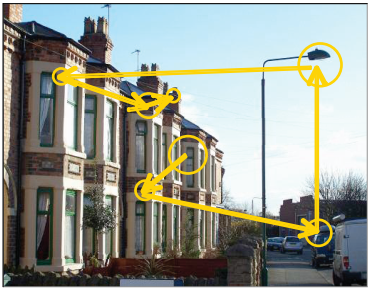
\includegraphics[width=.8\linewidth]{scan1.png}
  \caption{}
  \label{fig:sfig21}
\end{subfigure}%
\begin{subfigure}{.33\textwidth}
  \centering
  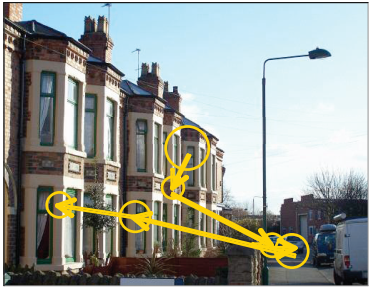
\includegraphics[width=.8\linewidth]{scan2.png}
  \caption{}
  \label{fig:sfig22}
\end{subfigure}
\begin{subfigure}{.33\textwidth}
  \centering
  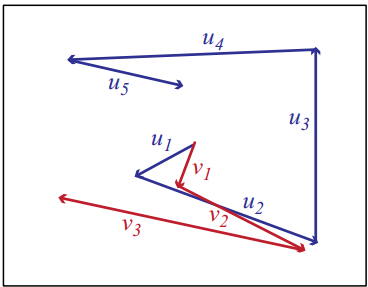
\includegraphics[width=.8\linewidth]{simple.png}
  \caption{}
  \label{fig:sfig23}
\end{subfigure}
\caption{(a) Human scanpath (b) Another scanpath from another human observer or scanpath generated by a model (c) Scanpaths in (a) and (b) simplified and temporaly aligned using MultiMatch. (\cite{Anderson2015} ) }
\label{fig:fig2}
\end{figure}

\begin{figure}[h]
    \centering
    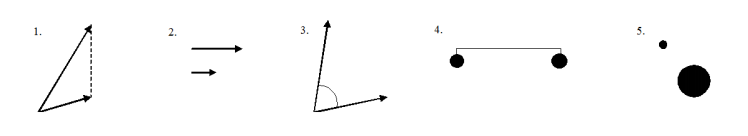
\includegraphics[scale=0.5]{multimatch}
    \caption{The five similarity metrics of MultiMatch. 1. vector, 2. length, 3. direction, 4. position and 5. duration  (\cite{7ccdec072dc945c4a0138a73aedd0132} )}
    \label{fig:MultiMatch}
\end{figure}
\newpage
\section{Results}
The table below shows the performance our model in comparison to what can be achieved by using one human scanpath to predict another and a random baseline. As we can see, our model outperforms the random baseline and for most of the metrics, it is close to the performance of using one other human scanpath to predict another. The research was conducted with in a seven week period for six units of credit
\begin{center}
\begin{tabular}{ |c|c|c|c|c|c|} 
 \hline
  & Vector & Length & Direction & Position & Duration \\ 
  \hline
  With Self & 1.0 & 1.0 & 1.0 & 1.0 & 1.0\\
 \hline
 
 Other Subject &  0.8801 & 0.7083 & 0.8864 & 0.8520 & 0.6525\\ 
 \hline
 Model Prediction &0.8560&0.6163&0.8667& 0.7898& 0.6481\\
 \hline
 Random Baseline & 0.7739 & 0.6061 & 0.7365 & 0.6882 & 0.5947\\
 \hline
\end{tabular}
\end{center}

%\begin{figure}
%\begin{subfigure}{1\textwidth}
  %\centering
  %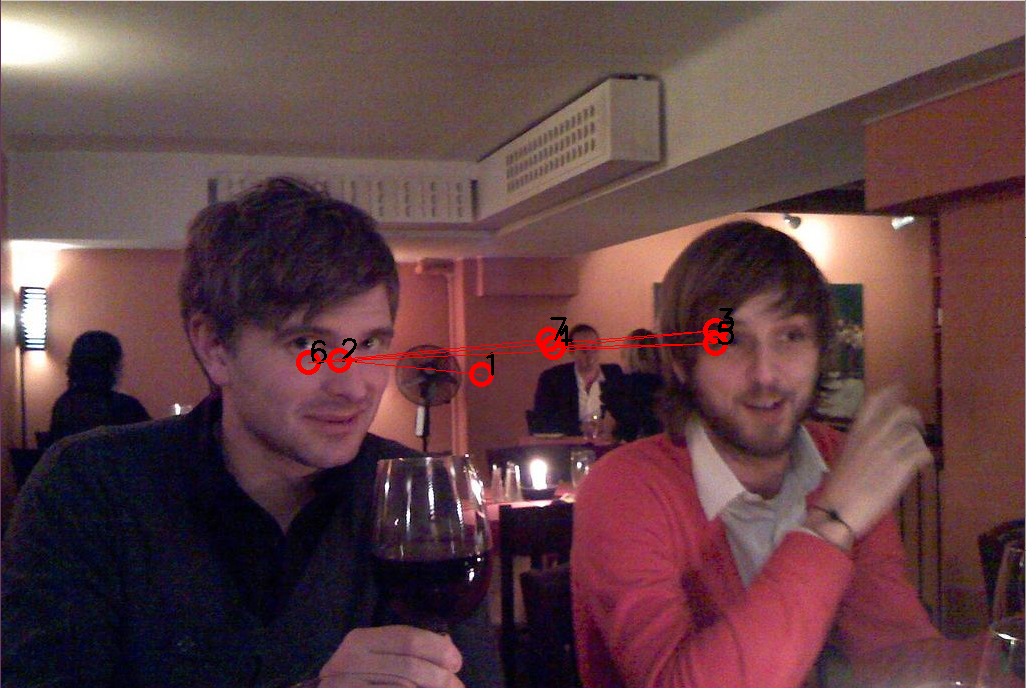
\includegraphics[width=.75\linewidth]{1.png}
  %\caption{}
  %\label{fig:1}
%\end{subfigure}
%\begin{subfigure}{1\textwidth}
 % \centering
  %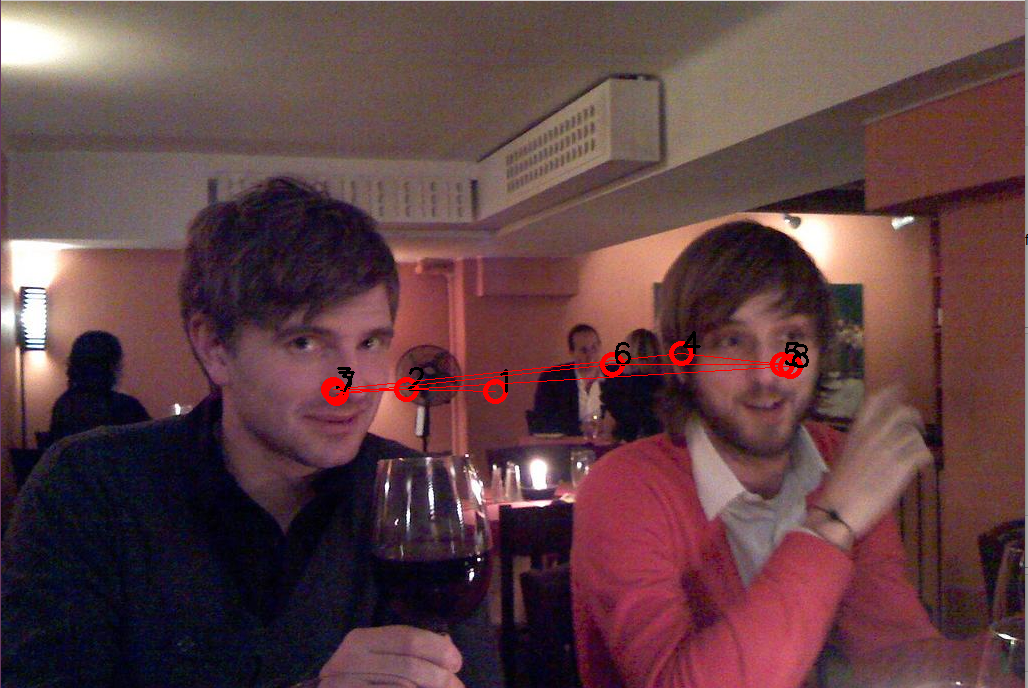
\includegraphics[width=.75\linewidth]{2.png}
% \caption{}
% \label{fig:2}
%\end{subfigure}
%\begin{subfigure}{1\textwidth}
%  \centering
%  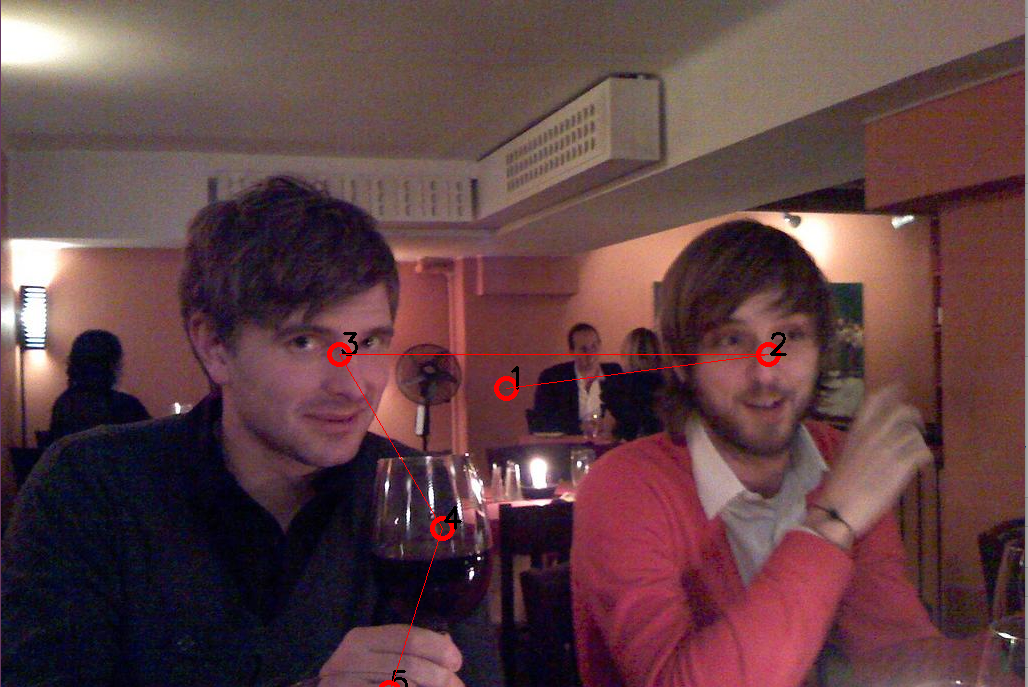
\includegraphics[width=.75\linewidth]{3.png}
%  \caption{}
%  \label{fig:3}
%\end{subfigure}
%\caption{(a) Human scanpath, (b) Predicted scanpath }
%\label{fig:final}
%\end{figure}


%\label{fig:fig2}
\begin{figure}
\begin{tabular}{cccc}
\subcaptionbox{Subject 1 scanpath}{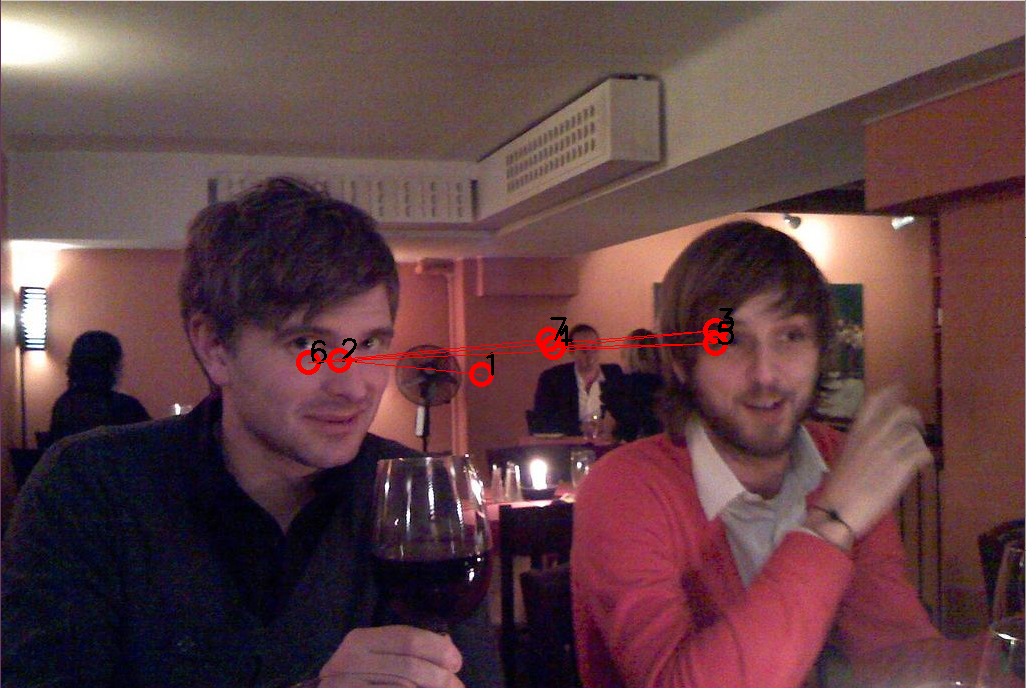
\includegraphics[width = 1.5in]{1.png}} &
\subcaptionbox{Subject 2 scanpath}{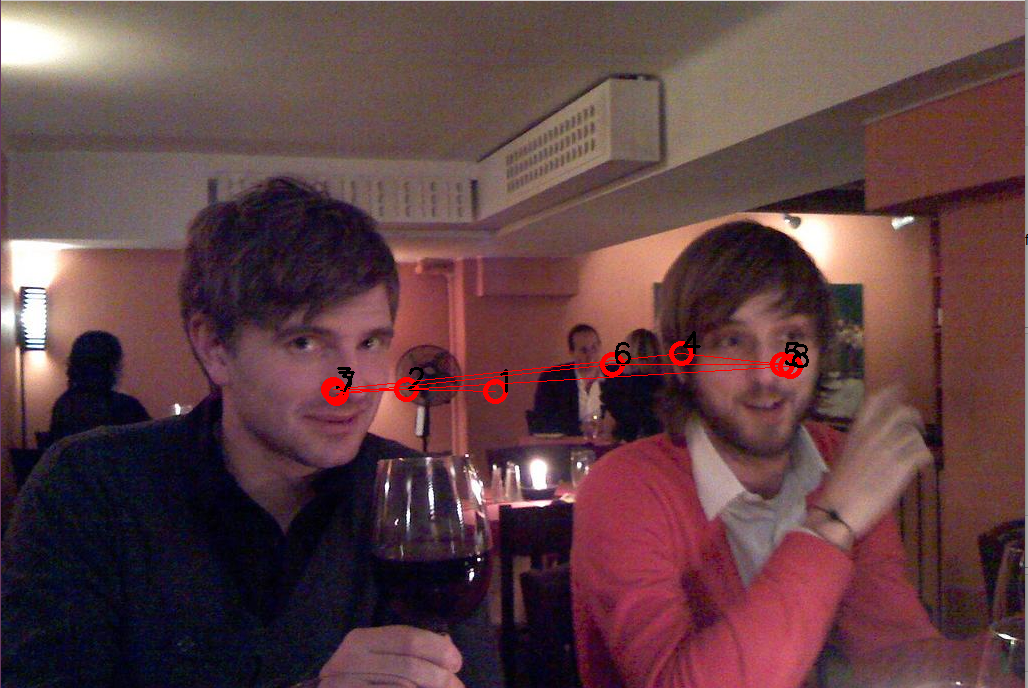
\includegraphics[width = 1.5in]{2.png}} &
\subcaptionbox{Subject 3 scanpath}{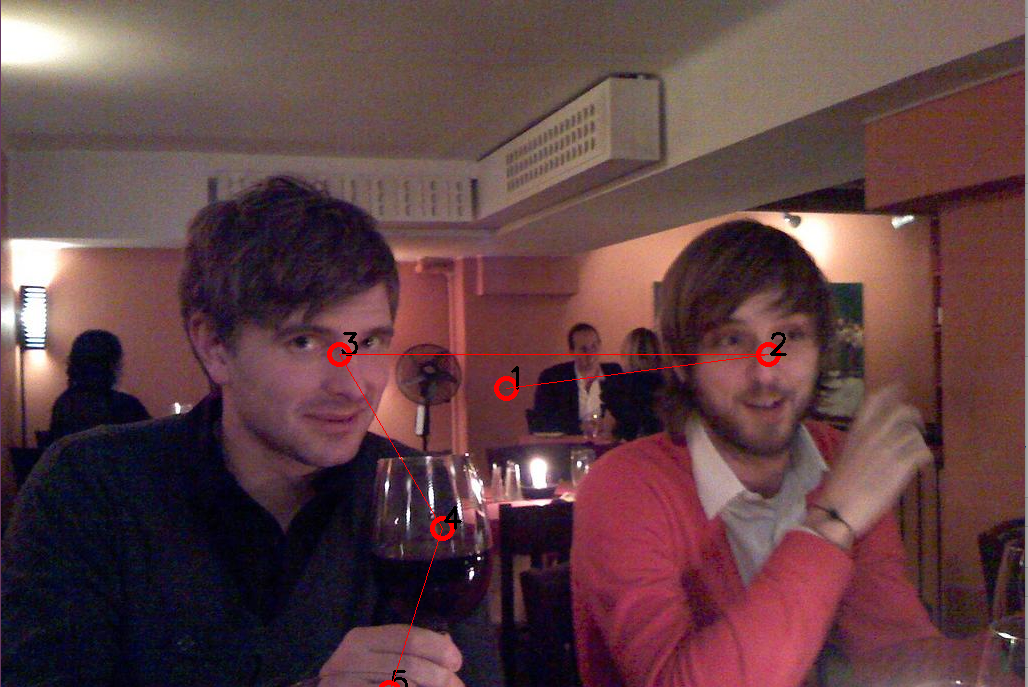
\includegraphics[width = 1.5in]{3.png}} &
\subcaptionbox{Subject 4 scanpath}{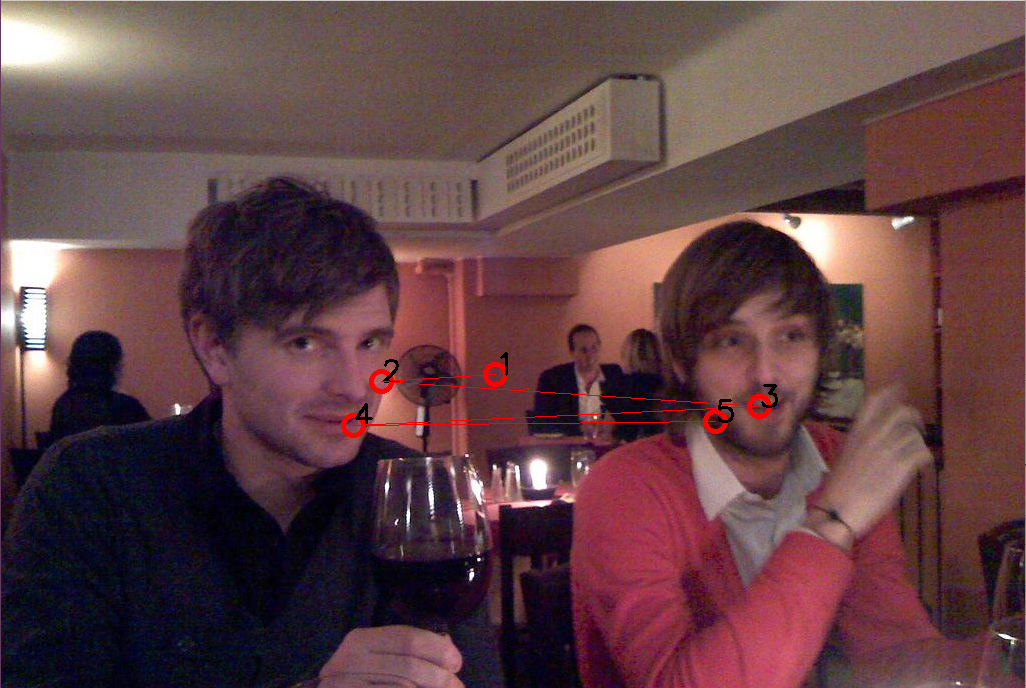
\includegraphics[width = 1.5in]{4.png}}\\
\subcaptionbox{Subject 5 scanpath}{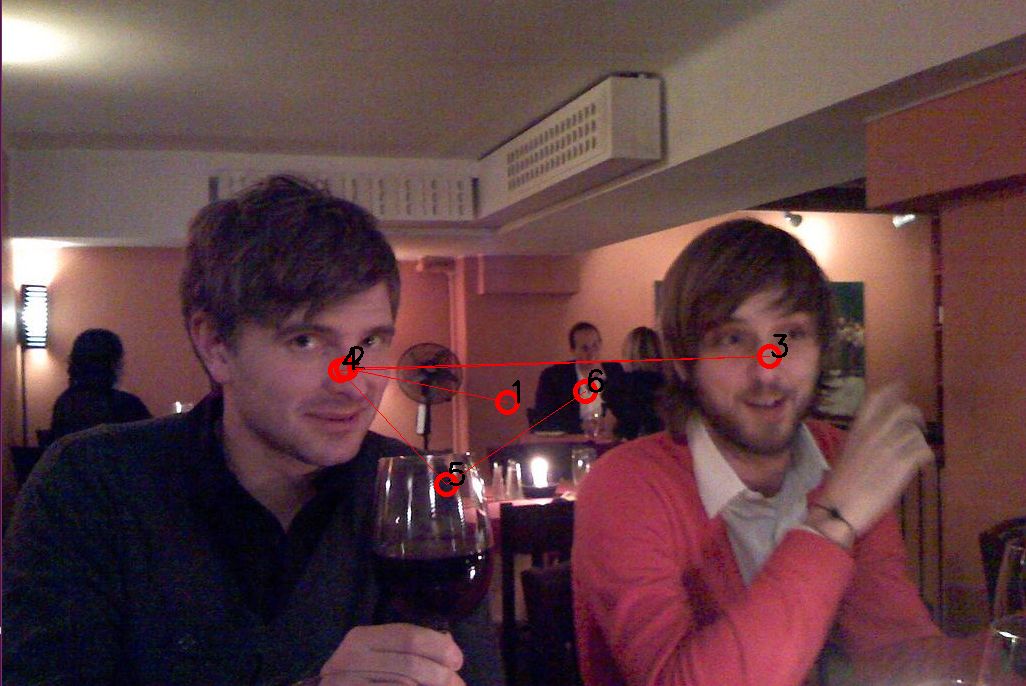
\includegraphics[width = 1.5in]{5.png}} &
\subcaptionbox{Subject 6 scanpath}{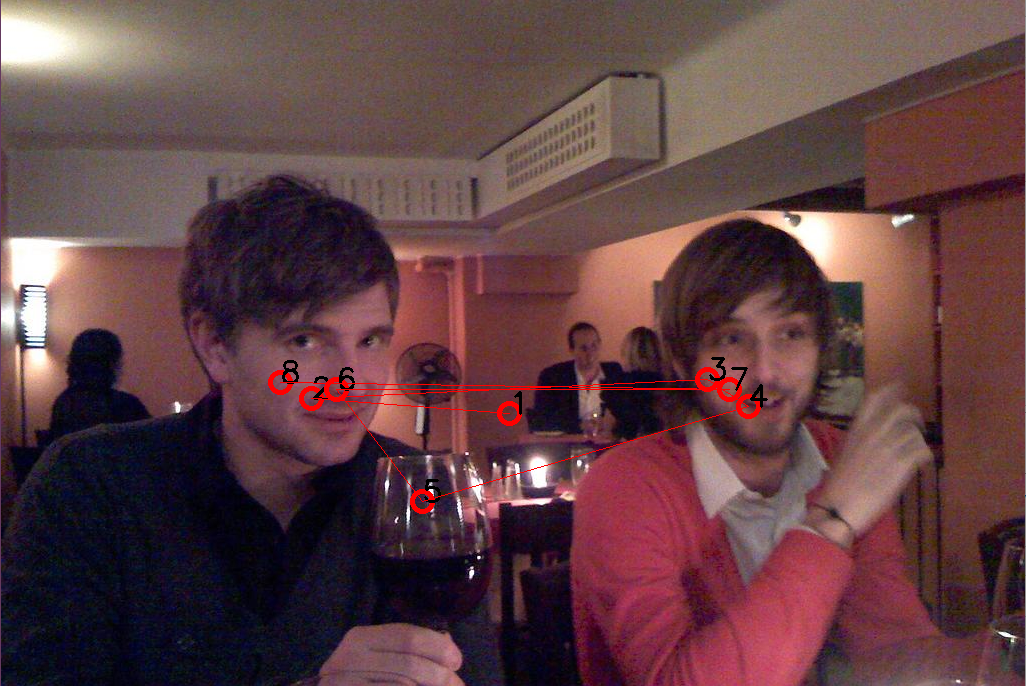
\includegraphics[width = 1.5in]{6.png}} &
\subcaptionbox{Subject 7 scanpath}{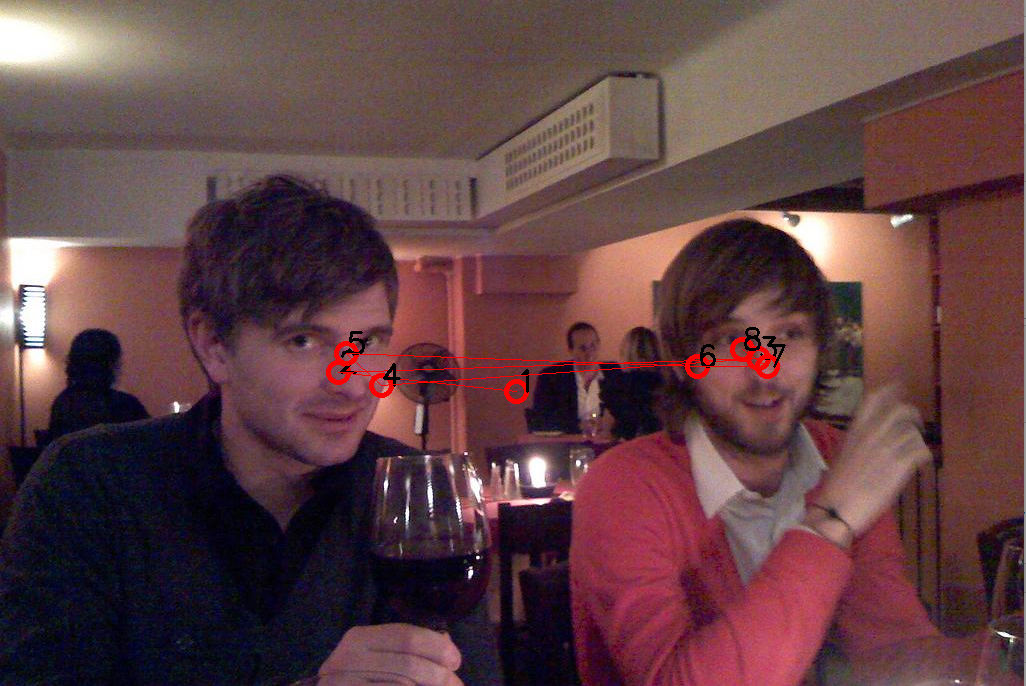
\includegraphics[width = 1.5in]{7.png}} &
\subcaptionbox{Subject 8 scanpath}{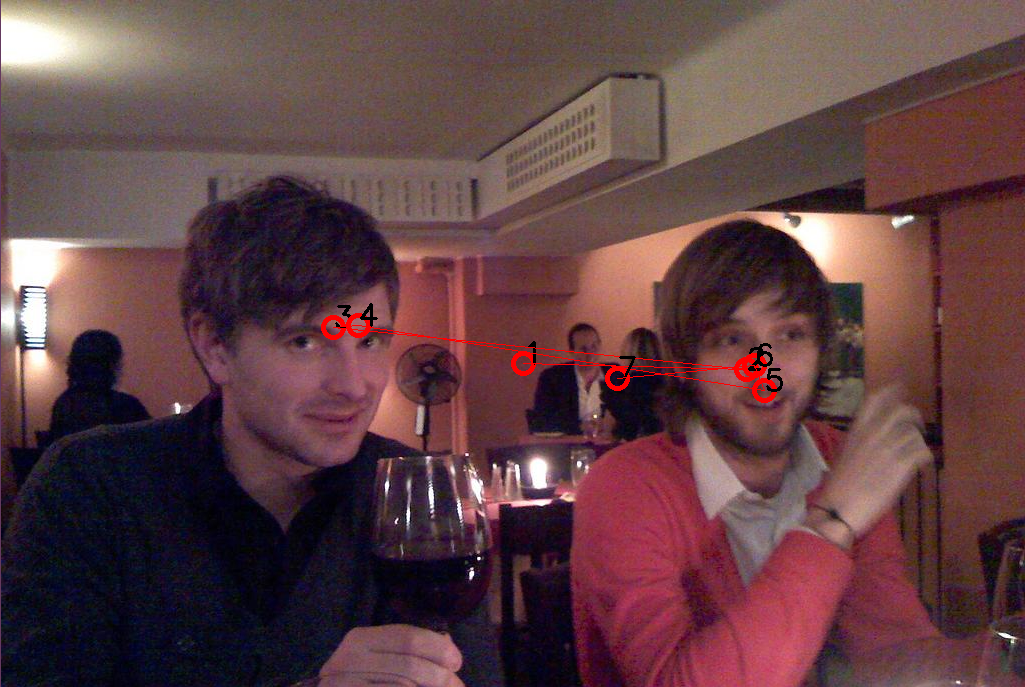
\includegraphics[width = 1.5in]{8.png}}\\
\subcaptionbox{Subject 9 scanpath}{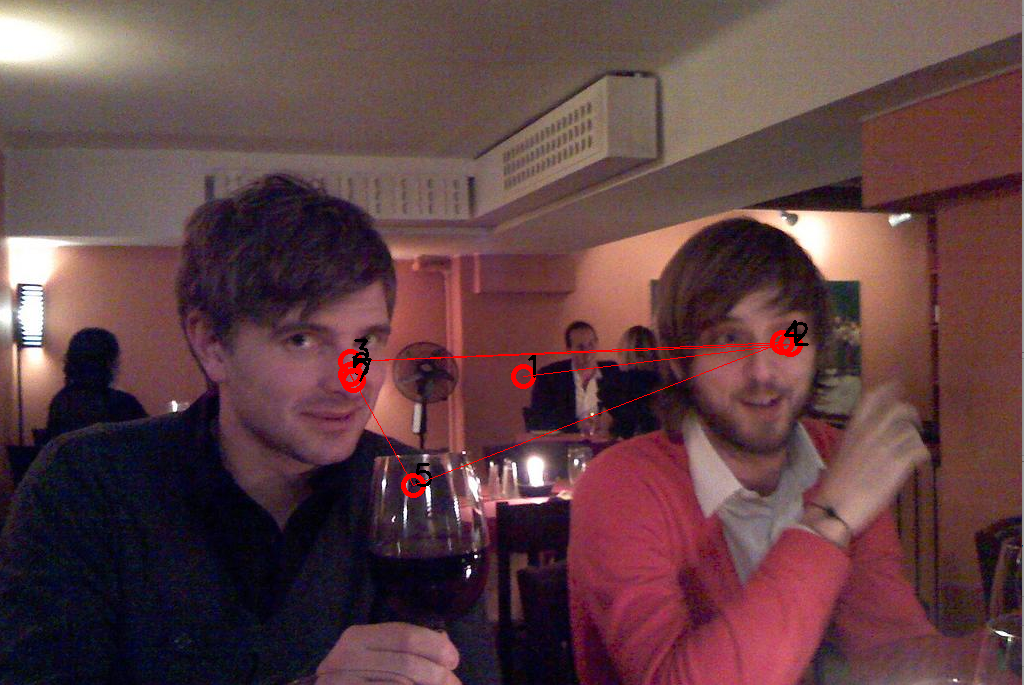
\includegraphics[width = 1.5in]{9.png}} &
\subcaptionbox{Subject 10 scanpath}{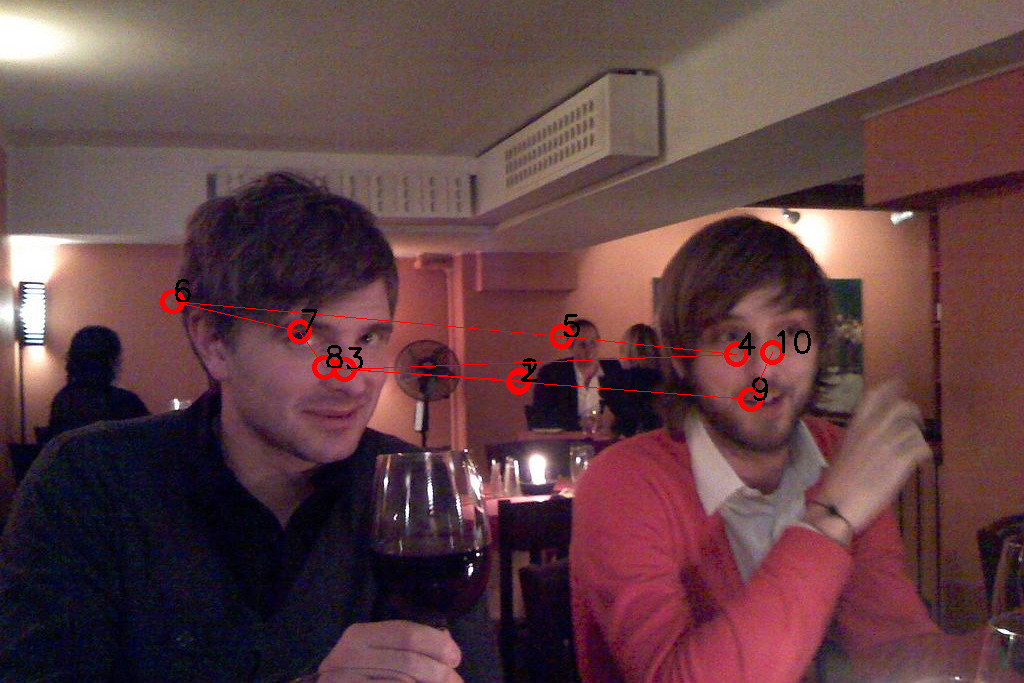
\includegraphics[width = 1.5in]{10.png}} &
\subcaptionbox{Subject 11 scanpath}{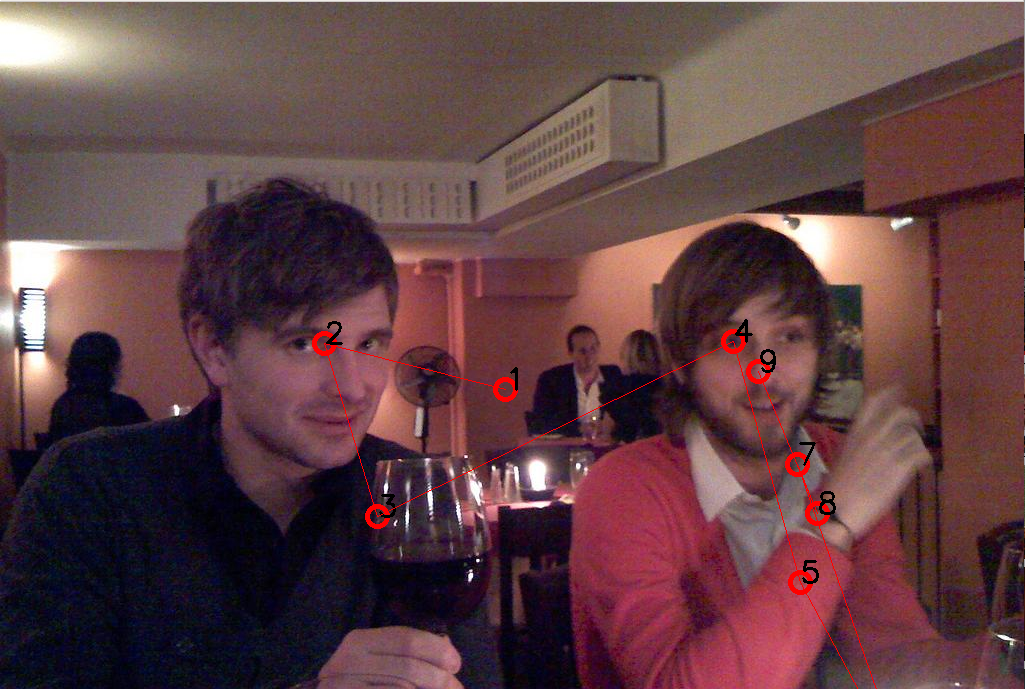
\includegraphics[width = 1.5in]{11.png}} &
\subcaptionbox{Subject 12 scanpath}{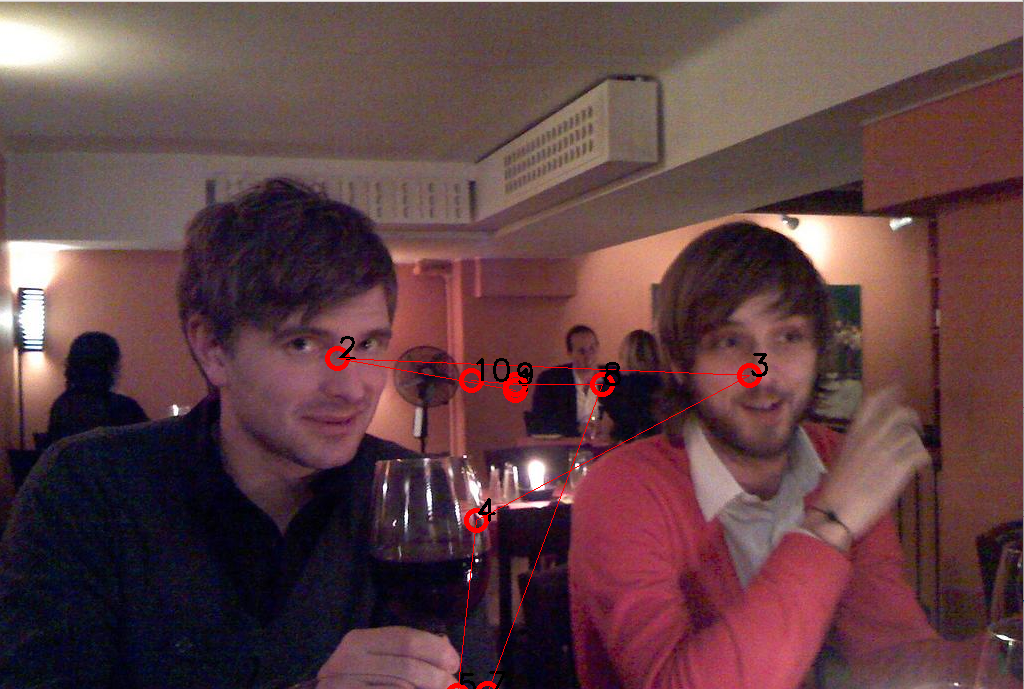
\includegraphics[width = 1.5in]{12.png}}\\
\subcaptionbox{Subject 13 scanpath}{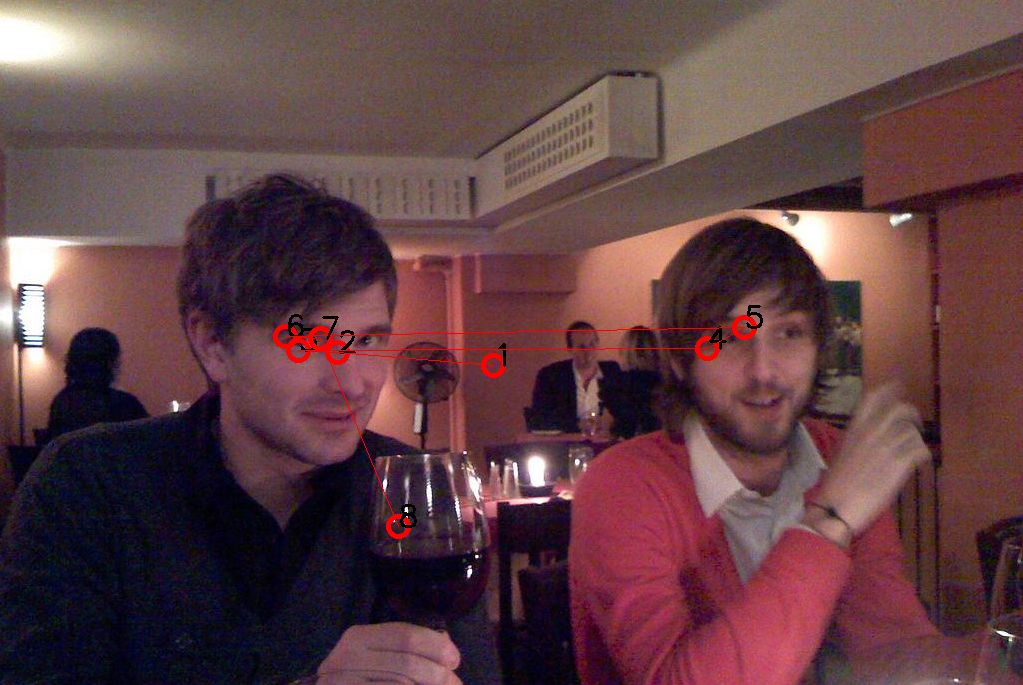
\includegraphics[width = 1.5in]{13.png}} &
\subcaptionbox{Subject 14 scanpath}{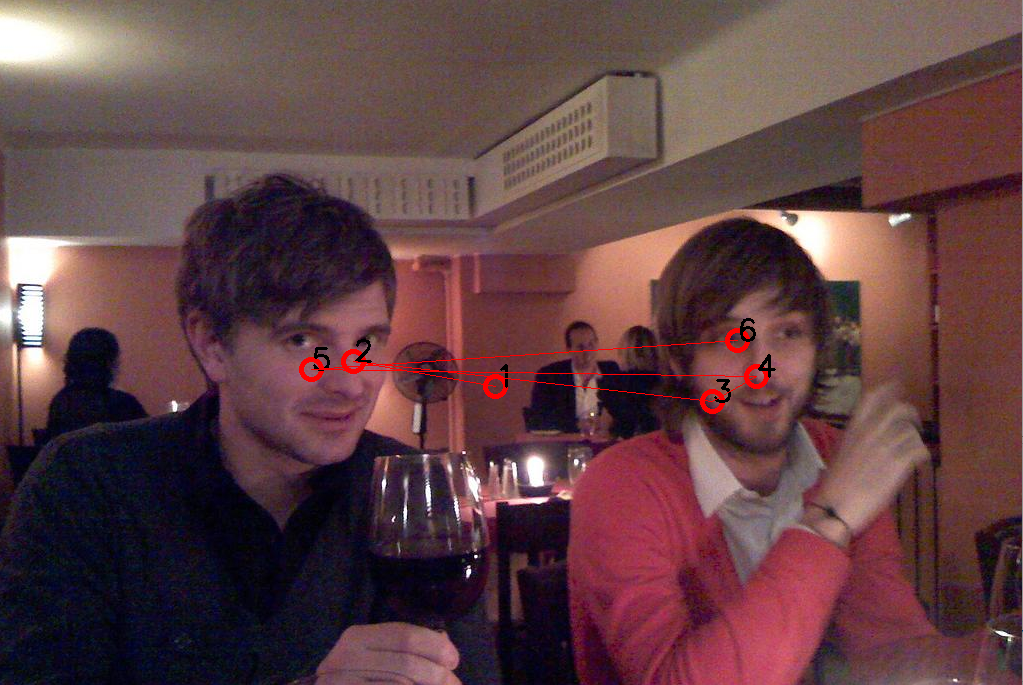
\includegraphics[width = 1.5in]{14.png}} &
\subcaptionbox{Subject 15 scanpath}{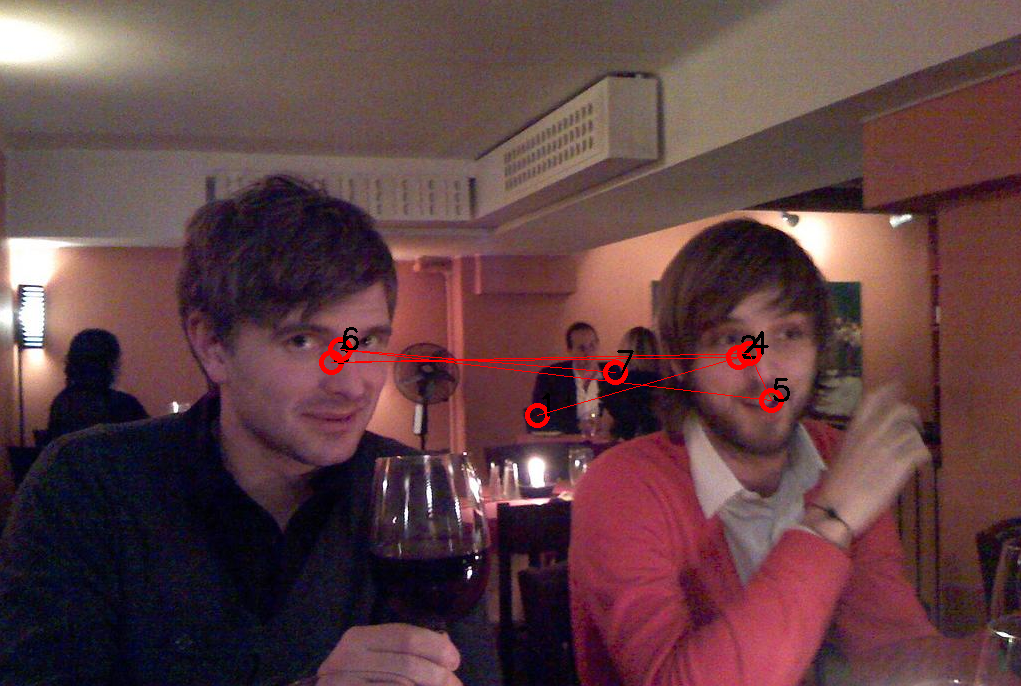
\includegraphics[width = 1.5in]{15.png}} &
\subcaptionbox{Our prediction}{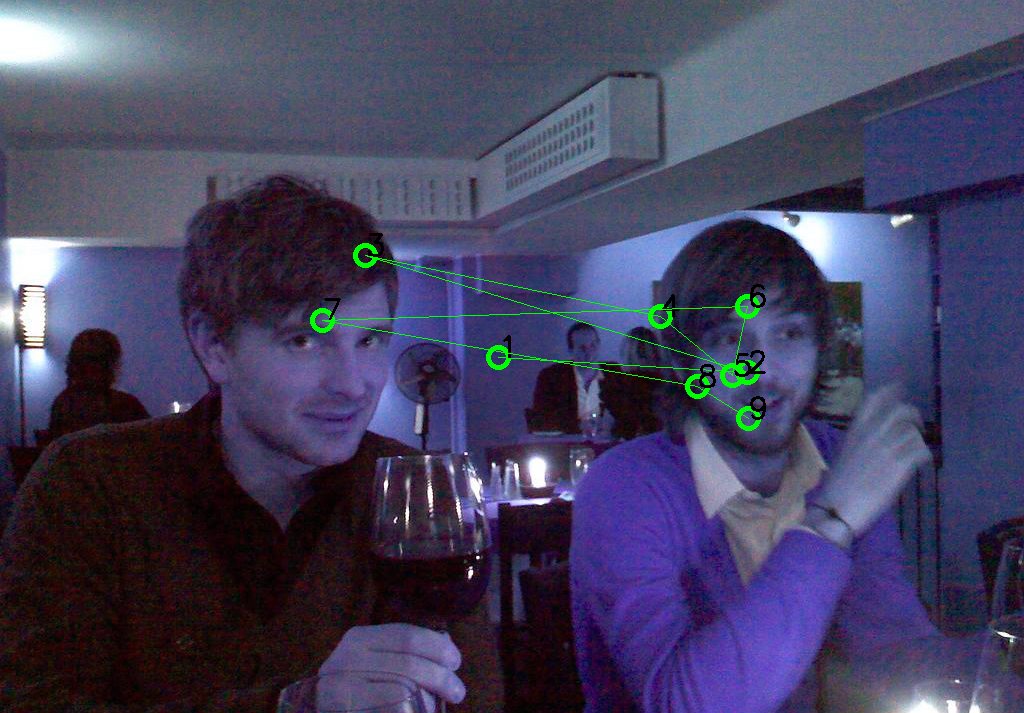
\includegraphics[width = 1.5in]{prediction.png}}
\end{tabular}
\caption{(a)-(o) human scanpaths for the same stimulus. (p) is our prediction for the same stimulus}
\end{figure}

\section{Conclusion and Future Works}
We have proposed a generative model based on a deep recurrent architecture that
predicts human visual scan-path, gaze sequences, for a given image in  free viewing task. The model is trained end to end with real-world human eye-tracking data  to maximize the likelihood of desired gaze sequence given a downsampled version of an image. We have shown that this model has close performance to using one  human scanpath to predict another's on the different similarity metrics of MultiMatch and outperforms the random baseline. 

In the future, we can do a number of things to improve the current performance of our model. First, we can try to overcome the the over-fitting problem by using different data augmentation techniques and implementing the different regularization techniques for the LSTM part described in \cite{DBLP:journals/corr/abs-1708-02182}. Second, training the Encoder from scratch and seeing if that will result in a better feature extractor. If the first two do not work, we can try modifying our network architecture to one with an attention mechanism similar to the one described in \cite{DBLP:journals/corr/XuBKCCSZB15}. After experimenting with the aforementioned model improvement strategies, we would like compare it with other scanpath generation methods on the same dataset. 

\bibliography{11785_project}
\bibliographystyle{11785_project}

\end{document}
